\chapter{Implementacja algorytmu KLT}
\label{cha:implementacjaalgorytmuklt}

Jak opisywano w sekcji \ref{sec:wyborimplementowanegoalgorytmu} najlepiej z zadaniem śledzenia w modelu programowym poradził sobie algorytm KLT. W związku z tym postanowiono przeprowadzić próbę jego implementacji w układzie Zynq. Należy zauważyć, że celem autora było zaimplementowanie jak największej części algorytmu w logice rekonfigurowalnej, aby zmniejszyć ilość obliczeń potrzebnych do wykonania w procesorze oraz jak najwięcej z nich wykonywać równolegle. W efekcie system ma działać szybko, wymagać małej ilości energii oraz będzie go można łatwo rozbudować lub zmienić zamieniając tylko odpowiednie moduły w diagramie blokowym programu \textit{Vivado}.

\paragraph*{}
Metoda śledzenia KLT działa na obrazie w skali szarości. Konwersję przeprowadzamy tak jak dla metody Mean-shift, z użyciem wzoru \ref{eq:grayscale}. Zgodnie z przebiegiem algorytmu przestawionym w sekcji \ref{sec:klt}, działanie algorytmu rozpoczyna się od wyboru punktów charakterystycznych spełniających warunek na wartości własne hesjanu. Aby to zrobić najpierw musimy wyliczyć gradient obrazu wejściowego. Jest on obliczany jako konwolucja dwuwymiarowa obrazu wejściowego z następującymi maskami:
\begin{equation}
M_x=
	\begin{bmatrix}
	-1 & 0 & 1
	\end{bmatrix}
\end{equation}
\begin{equation}
M_y=
	\begin{bmatrix}
	-1 \\
	0 \\
	1
	\end{bmatrix}
\end{equation}
Wyniki powyższych splotów są następnie podnoszone do kwadratów i mnożone przez siebie. W wyniku otrzymuje się macierz hesjanu dla aktualnego piksela. Zdecydowano, że powyższe wartości będą wyliczane dla całego obrazu w sposób potokowy. Aby to zrealizować należy zaimplementować również linię opóźniającą wartości pikseli oraz sygnały synchronizacyjne z użyciem pamięci BRAM, gdyż do wykonania powyższych działań potrzebujemy wartości pikseli z wcześniejszych linii obrazu wejściowego. Należy również wyznaczyć latencję użytych sumatorów i mnożarek, by opóźnić sygnały synchronizacyjne o odpowiednią liczbę taktów zegara.

\paragraph*{}
Aby wyznaczyć punkty charakterystyczne następnie należy wyliczone wartości hesjanów poddać filtracji filtrem Gaussowskim. Jądro dwuwymiarowego filtru Gaussowskiego o wymiarze \(3\)x\(3\), wartości oczekiwanej równej \((0,0)\) i odchyleniu standardowym równym \(1\) wynosi:
\begin{equation}
\label{eq:gauss}
M_G=
	\begin{bmatrix}
	0.0751 & 0.1238 & 0.0751\\
	0.1238 & 0.2042 & 0.1238\\
	0.0751 & 0.1238 & 0.0751
	\end{bmatrix}
\end{equation}
Zwykły filtr Gaussowski wymagałby jednak dużej ilości zasobów (kilku mnożarek), więc postanowiono zaimplementować tzw. dyskretną wersję powyższego jądra, która ma postać \cite{Benda}:
\begin{equation}
M_G=\frac{1}{16} \cdot
	\begin{bmatrix}
	1 & 2 & 1\\
	2 & 4 & 2\\
	1 & 2 & 1
	\end{bmatrix}
\end{equation}
Powyższy filtr w porównaniu do \ref{eq:gauss} nie wymaga użycia mnożarek. Zamiast tego wykorzystujemy przesunięcia bitowe. Implementacja wymaga kolejnej linii opóźniającej oraz dodatkowego opóźnienia sygnałów synchronizacyjnych.

\paragraph*{}
Na podstawie wyników opisanego powyżej splotu obliczamy funkcję celu, czyli wartość mniejszej wartości własnej hesjanu. Hesjan ma postać:
\begin{equation}
H=
	\begin{bmatrix}
	H_{xx} & H_{xy}\\
	H_{xy} & H_{yy}
	\end{bmatrix}
\end{equation}
Wyznaczono analitycznie jego wartości własne.
\begin{equation}
\begin{vmatrix}
H_{xx}-\lambda & H_{xy} \\
X_{xy} & H_{yy}-\lambda
\end{vmatrix}=0
\end{equation}
\begin{equation}
(H_{xx}-\lambda)(H_{yy}-\lambda)-H_{xy}^2=0
\end{equation}
\begin{equation}
\lambda^2-\lambda(H_{xx}+H_{yy})+H_{xx}H_{yy}-H_{xy}^2=0
\end{equation}
\begin{equation}
\label{eq:delta}
\Delta=(H_{xx}-H_{yy})^2+4H_{xy}^2 \geqslant 0
\end{equation}
Mniejsza z jego wartości własnych wynosi więc:
\begin{equation}
\label{eq:lambda}
\lambda=\frac{H_{xx}+H_{yy}-\sqrt{\Delta}}{2}
\end{equation}
Piksele dla których obliczona wartość funkcji celu jest największa są punktami charakterystycznymi. Ze wzorów \ref{eq:delta} i \ref{eq:lambda} widać, że obliczenie wartości własnej wymagać będzie modułów mnożarki, sumatorów oraz obliczania pierwiastka podanej wartości. Obliczenia te zostały zrealizowane za pomocą modułów dostępnych w programie \textit{Vivado}.

\begin{figure}[H]
	\centering
	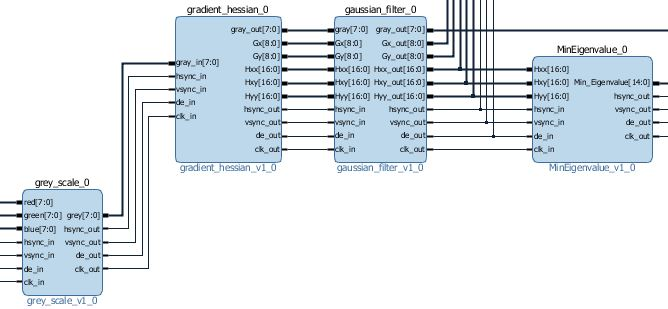
\includegraphics[width=4in]{mineig_vivado.jpg}
	\captionsource{Fragment schematu blokowego, realizujący opisane powyżej operacje.}{Własne}
\end{figure}

\begin{figure}[H]
	\centering
	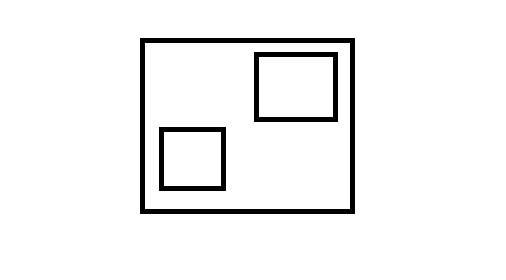
\includegraphics[width=4in]{test.png}
	\captionsource{Przykładowy obraz wejściowy.}{Własne}
\end{figure}

\begin{figure}[H]
	\centering
	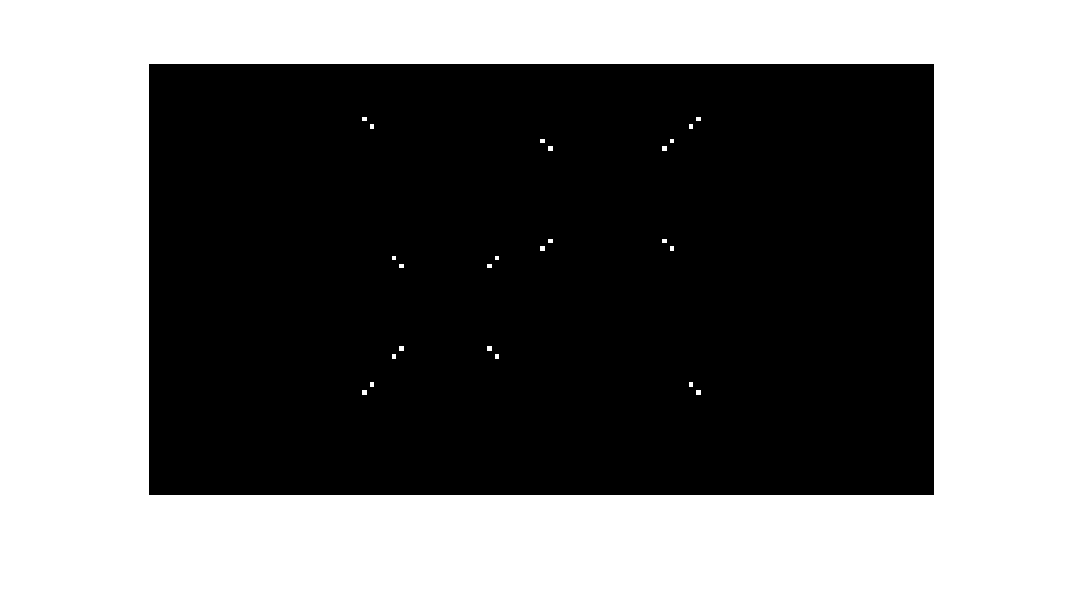
\includegraphics[width=4in]{test_out.eps}
	\captionsource{Obraz wyjściowy odpowiadający wejściowemu.}{Własne}
\end{figure}

Nie udało się dokończyć implementacji algorytmu KLT. Potrzeba jeszcze zaimplementować operacje realizujące śledzenie okna wokół wybranych punktów charakterystycznych, a więc obliczające wartość przesunięcia z równania \ref{eq:dp_klt} oraz iteracyjne wyznaczanie przesunięcia za pomocą wspomnianego wzoru.